% 若编译失败,且生成 .synctex(busy) 辅助文件,可能有两个原因:
% 1. 需要插入的图片不存在:Ctrl + F 搜索 'figure' 将这些代码注释/删除掉即可
% 2. 路径/文件名含中文或空格:更改路径/文件名即可

% --------------------- 文章宏包及相关设置 --------------------- %
% >> ------------------ 文章宏包及相关设置 ------------------ << %
% 设定文章类型与编码格式
\documentclass[UTF8]{article}		

% 物理实验报告所需的其它宏包
\usepackage{ulem}   % \uline 下划线支持
\usepackage{circuitikz} % 电路图 tikz 支持
\usepackage{pdfpages}   % 用于导入 pdf 文件

% 本 .tex 专属的宏定义
    \def\V{\ \mathrm{V}}
    \def\uV{\ \mu\mathrm{V}}
    \def\mV{\ \mathrm{mV}}
    \def\K{\ \mathrm{K}}
    \def\kV{\ \mathrm{KV}}
    \def\KV{\ \mathrm{KV}}
    \def\MV{\ \mathrm{MV}}
    \def\uA{\ \mu\mathrm{A}}
    \def\mA{\ \mathrm{mA}}
    \def\A{\ \mathrm{A}}
    \def\kA{\ \mathrm{KA}}
    \def\KA{\ \mathrm{KA}}
    \def\MA{\ \mathrm{MA}}
    \def\O{\ \Omega}
    \def\mO{\ \Omega}
    \def\kO{\ \mathrm{K}\Omega}
    \def\KO{\ \mathrm{K}\Omega}
    \def\MO{\ \mathrm{M}\Omega}
    \def\Hz{\ \mathrm{Hz}}
    \def\uF{\ \mu\mathrm{F}}
    \def\mF{\ \mathrm{mF}}
    \def\F{\ \mathrm{F}}
    \def\Re{\mathrm{\,Re}\,}
    \def\Im{\mathrm{\,Im}\,}
    \def\sinc{\mathrm{\,sinc}\,}

% 自定义宏定义
    \def\N{\mathbb{N}}
    \def\F{\mathbb{F}}
    \def\Z{\mathbb{Z}}
    \def\Q{\mathbb{Q}}
    \def\R{\mathbb{R}}
    \def\C{\mathbb{C}}
    \def\T{\mathbb{T}}
    \def\S{\mathbb{S}}
    %\def\A{\mathbb{A}}
    \def\I{\mathscr{I}}
    \def\d{\mathrm{d}}
    \def\p{\partial}


% 导入基本宏包
    \usepackage[UTF8]{ctex}     % 设置文档为中文语言
    \usepackage{hyperref}  % 宏包:自动生成超链接 (此宏包与标题中的数学环境冲突)
    \hypersetup{
        colorlinks=true,    % false:边框链接 ; true:彩色链接
        citecolor={blue},    % 文献引用颜色
        linkcolor={blue},   % 目录 (我们在目录处单独设置),公式,图表,脚注等内部链接颜色
        urlcolor={orange},    % 网页 URL 链接颜色,包括 \href 中的 text
        % cyan 浅蓝色 
        % magenta 洋红色
        % yellow 黄色
        % black 黑色
        % white 白色
        % red 红色
        % green 绿色
        % blue 蓝色
        % gray 灰色
        % darkgray 深灰色
        % lightgray 浅灰色
        % brown 棕色
        % lime 石灰色
        % olive 橄榄色
        % orange 橙色
        % pink 粉红色
        % purple 紫色
        % teal 蓝绿色
        % violet 紫罗兰色
    }
    % \usepackage{docmute}    % 宏包:子文件导入时自动去除导言区,用于主/子文件的写作方式,\include{./51单片机笔记}即可。注:启用此宏包会导致.tex文件capacity受限。
    \usepackage{amsmath}    % 宏包:数学公式
    \usepackage{mathrsfs}   % 宏包:提供更多数学符号
    \usepackage{amssymb}    % 宏包:提供更多数学符号
    \usepackage{pifont}     % 宏包:提供了特殊符号和字体
    \usepackage{extarrows}  % 宏包:更多箭头符号 
    \usepackage{multicol}   % 宏包:支持多栏 

% 文章页面margin设置
    \usepackage[a4paper]{geometry}
        \geometry{top=0.75in}
        \geometry{bottom=0.75in}
        \geometry{left=0.75in}
        \geometry{right=0.75in}   % 设置上下左右页边距
        \geometry{marginparwidth=1.75cm}    % 设置边注距离(注释、标记等)

% 配置数学环境
    \usepackage{amsthm} % 宏包:数学环境配置
    % theorem-line 环境自定义
        \newtheoremstyle{MyLineTheoremStyle}% <name>
            {11pt}% <space above>
            {11pt}% <space below>
            {\kaishu}% <body font> 默认使用正文字体, \kaishu 为楷体
            {}% <indent amount>
            {\bfseries}% <theorem head font> 设置标题项为加粗
            {:\ \ }% <punctuation after theorem head>
            {.5em}% <space after theorem head>
            {\textbf{#1}\thmnumber{#2}\ \ (\,\textbf{#3}\,)}% 设置标题内容顺序
        \theoremstyle{MyLineTheoremStyle} % 应用自定义的定理样式
        \newtheorem{LineTheorem}{Theorem.\,}
    % theorem-block 环境自定义
        \newtheoremstyle{MyBlockTheoremStyle}% <name>
            {11pt}% <space above>
            {11pt}% <space below>
            {\kaishu}% <body font> 使用默认正文字体
            {}% <indent amount>
            {\bfseries}% <theorem head font> 设置标题项为加粗
            {:\\ \indent}% <punctuation after theorem head>
            {.5em}% <space after theorem head>
            {\textbf{#1}\thmnumber{#2}\ \ (\,\textbf{#3}\,)}% 设置标题内容顺序
        \theoremstyle{MyBlockTheoremStyle} % 应用自定义的定理样式
        \newtheorem{BlockTheorem}[LineTheorem]{Theorem.\,} % 使用 LineTheorem 的计数器
    % definition 环境自定义
        \newtheoremstyle{MySubsubsectionStyle}% <name>
            {11pt}% <space above>
            {11pt}% <space below>
            {}% <body font> 使用默认正文字体
            {}% <indent amount>
            {\bfseries}% <theorem head font> 设置标题项为加粗
            {:\\ \indent}% <punctuation after theorem head>
            {0pt}% <space after theorem head>
            {\textbf{#3}}% 设置标题内容顺序
        \theoremstyle{MySubsubsectionStyle} % 应用自定义的定理样式
        \newtheorem{definition}{}

%宏包:有色文本框(proof环境)及其设置
    \usepackage{xcolor}    %设置插入的文本框颜色
    \usepackage[strict]{changepage}     % 提供一个 adjustwidth 环境
    \usepackage{framed}     % 实现方框效果
        \definecolor{graybox_color}{rgb}{0.95,0.95,0.96} % 文本框颜色。修改此行中的 rgb 数值即可改变方框纹颜色,具体颜色的rgb数值可以在网站https://colordrop.io/ 中获得。(截止目前的尝试还没有成功过,感觉单位不一样)(找到喜欢的颜色,点击下方的小眼睛,找到rgb值,复制修改即可)
        \newenvironment{graybox}{%
        \def\FrameCommand{%
        \hspace{1pt}%
        {\color{gray}\vrule width 2pt}%
        {\color{graybox_color}\vrule width 4pt}%
        \colorbox{graybox_color}%
        }%
        \MakeFramed{\advance\hsize-\width\FrameRestore}%
        \noindent\hspace{-4.55pt}% disable indenting first paragraph
        \begin{adjustwidth}{}{7pt}%
        \vspace{2pt}\vspace{2pt}%
        }
        {%
        \vspace{2pt}\end{adjustwidth}\endMakeFramed%
        }

% 外源代码插入设置
    % matlab 代码插入设置
    \usepackage{matlab-prettifier}
        \lstset{style=Matlab-editor}    % 继承 matlab 代码高亮 , 此行不能删去
    \usepackage[most]{tcolorbox} % 引入tcolorbox包 
    \usepackage{listings} % 引入listings包
        \tcbuselibrary{listings, skins, breakable}
        \newfontfamily\codefont{Consolas} % 定义需要的 codefont 字体
        \lstdefinestyle{MatlabStyle_inc}{   % 插入代码的样式
            language=Matlab,
            basicstyle=\footnotesize\ttfamily\codefont,    % ttfamily 确保等宽 
            breakatwhitespace=false,
            breaklines=true,
            captionpos=b,
            keepspaces=true,
            numbers=left,
            numbersep=15pt,
            showspaces=false,
            showstringspaces=false,
            showtabs=false,
            tabsize=2,
            xleftmargin=15pt,   % 左边距
            %frame=single, % single 为包围式单线框
            frame=shadowbox,    % shadowbox 为带阴影包围式单线框效果
            %escapeinside=``,   % 允许在代码块中使用 LaTeX 命令 (此行无用)
            %frameround=tttt,    % tttt 表示四个角都是圆角
            framextopmargin=0pt,    % 边框上边距
            framexbottommargin=0pt, % 边框下边距
            framexleftmargin=5pt,   % 边框左边距
            framexrightmargin=5pt,  % 边框右边距
            rulesepcolor=\color{red!20!green!20!blue!20}, % 阴影框颜色设置
            %backgroundcolor=\color{blue!10}, % 背景颜色
        }
        \lstdefinestyle{MatlabStyle_src}{   % 插入代码的样式
            language=Matlab,
            basicstyle=\small\ttfamily\codefont,    % ttfamily 确保等宽 
            breakatwhitespace=false,
            breaklines=true,
            captionpos=b,
            keepspaces=true,
            numbers=left,
            numbersep=15pt,
            showspaces=false,
            showstringspaces=false,
            showtabs=false,
            tabsize=2,
        }
        \newtcblisting{matlablisting}{
            %arc=2pt,        % 圆角半径
            % 调整代码在 listing 中的位置以和引入文件时的格式相同
            top=0pt,
            bottom=0pt,
            left=-5pt,
            right=-5pt,
            listing only,   % 此句不能删去
            listing style=MatlabStyle_src,
            breakable,
            colback=white,   % 选一个合适的颜色
            colframe=black!0,   % 感叹号后跟不透明度 (为 0 时完全透明)
        }
        \lstset{
            style=MatlabStyle_inc,
        }

% table 支持
    \usepackage{booktabs}   % 宏包:三线表
    \usepackage{tabularray} % 宏包:表格排版
    \usepackage{longtable}  % 宏包:长表格

% figure 设置
    \usepackage{graphicx}  % 支持 jpg, png, eps, pdf 图片 
    \usepackage{svg}       % 支持 svg 图片
        \svgsetup{
            % 指向 inkscape.exe 的路径
            inkscapeexe = C:/aa_MySame/inkscape/bin/inkscape.exe, 
            % 一定程度上修复导入后图片文字溢出几何图形的问题
            inkscapelatex = false                 
        }
    \usepackage{subcaption} % 用于子图和小图注  

% 图表进阶设置
    \usepackage{caption}    % 图注、表注
        \captionsetup[figure]{name=图}  
        \captionsetup[table]{name=表}
        \captionsetup{
            labelfont=bf, % 设置标签为粗体
            textfont=bf,  % 设置文本为粗体
            font=small  
        }
    \usepackage{float}     % 图表位置浮动设置 
    \usepackage{etoolbox} % 用于保证图注表注的数学字符为粗体
        \AtBeginEnvironment{figure}{\boldmath} % 图注中的数学字符为粗体
        \AtBeginEnvironment{table}{\boldmath}  % 表注中的数学字符为粗体
        \AtBeginEnvironment{tabular}{\unboldmath}   % 保证表格中的数学字符不受额外影响

% 圆圈序号自定义
    \newcommand*\circled[1]{\tikz[baseline=(char.base)]{\node[shape=circle,draw,inner sep=0.8pt, line width = 0.03em] (char) {\bfseries #1};}}   % TikZ solution

% 列表设置
    \usepackage{enumitem}   % 宏包:列表环境设置
        \setlist[enumerate]{
            label=(\arabic*) ,   % 设置序号样式为加粗的 (1) (2) (3)
            ref=\arabic*, % 如果需要引用列表项,这将决定引用格式(这里仍然使用数字)
            itemsep=0pt, parsep=0pt, topsep=0pt, partopsep=0pt, leftmargin=3.5em} 
        \setlist[itemize]{itemsep=0pt, parsep=0pt, topsep=0pt, partopsep=0pt, leftmargin=3.5em}
        \newlist{circledenum}{enumerate}{1} % 创建一个新的枚举环境  
        \setlist[circledenum,1]{  
            label=\protect\circled{\arabic*}, % 使用 \arabic* 来获取当前枚举计数器的值,并用 \circled 包装它  
            ref=\arabic*, % 如果需要引用列表项,这将决定引用格式(这里仍然使用数字)
            itemsep=0pt, parsep=0pt, topsep=0pt, partopsep=0pt, leftmargin=3.5em
        }  

% 其它设置
    % 脚注设置
        \renewcommand\thefootnote{\ding{\numexpr171+\value{footnote}}}
    % 参考文献引用设置
        \bibliographystyle{unsrt}   % 设置参考文献引用格式为unsrt
        \newcommand{\upcite}[1]{\textsuperscript{\cite{#1}}}     % 自定义上角标式引用
    % 文章序言设置
        \newcommand{\cnabstractname}{序言}
        \newenvironment{cnabstract}{%
            \par\Large
            \noindent\mbox{}\hfill{\bfseries \cnabstractname}\hfill\mbox{}\par
            \vskip 2.5ex
            }{\par\vskip 2.5ex}

% 文章默认字体设置
    \usepackage{fontspec}   % 宏包:字体设置
        \setmainfont{SimSun}    % 设置中文字体为宋体字体
        \setCJKmainfont[AutoFakeBold=3]{SimSun} % 设置加粗字体为 SimSun 族,AutoFakeBold 可以调整字体粗细
        \setmainfont{Times New Roman} % 设置英文字体为Times New Roman

% 各级标题自定义设置
    \usepackage{titlesec}   
        % section标题自定义设置 
        \titleformat{\section}[hang]{\normalfont\Large\bfseries\boldmath}{\thesection}{8pt}{}
        % subsection 标题自定义设置
        \titleformat{\subsection}[hang]{\normalfont\large\bfseries\boldmath}{\thesubsection}{8pt}{}
        \titlespacing*{\subsection}{0pt}{10pt}{6pt} % 控制上下间距


% --------------------- 文章宏包及相关设置 --------------------- %
% >> ------------------ 文章宏包及相关设置 ------------------ << %


% ------------------------ 文章信息区 ------------------------ %
% ------------------------ 文章信息区 ------------------------ %
% 页眉页脚设置
\usepackage{fancyhdr}   %宏包:页眉页脚设置
    \pagestyle{fancy}
    \fancyhf{}
    \cfoot{\thepage}
    \renewcommand\headrulewidth{1pt}
    \renewcommand\footrulewidth{0pt}
    \rhead{\bfseries \large {\color{red} 分组序号: 2-05}}    
    \chead{《基础物理实验》实验报告,\ 丁毅,\ 2023K8009908031}
    \lhead{Ex.9 微波干涉 (2024.10.29)}

% 开始编辑文章

\begin{document}
\begin{center}\large
    \vspace*{-0.8cm}
    \noindent{\huge\bfseries《\ \ 基\ \ 础\ \ 物\ \ 理\ \ 实\ \ 验\ \ \ 》\ \ 实\ \ 验\ \ 报\ \ 告 }
    \\\vspace{0.1cm}
    \noindent{
    {\bfseries 
    实验名称:\uline{\hspace{2cm} 微波布拉格衍射 \hspace{2cm}}
    }\hspace{0.4cm}
    指导教师:\uline{\hspace{0.3cm}易栖如\ \ yiqiru@ucas.ac.cn\hspace{0.3cm}}
    }
    \\\vspace{0.1cm}
    \noindent
    {
    姓名:\uline{\,\,\,丁毅\,\,\,}\hspace{0.2cm}
    学号:\uline{\,\,\,{ 2023K8009908031}\,\,\,}\hspace{0.2cm}
    班级/专业:\uline{\,\,\,{2308/电子信息}\,\,\,}\hspace{0.2cm}
    分组序号:\uline{\,\,\,{2-05}\,\,\,}
    }
    \\\vspace{0.1cm}
    \noindent{
    实验日期:\uline{\,\,{ 2024.10.29}\,\,}\hspace{0.2cm}
    实验地点:\uline{\,\,\,教学楼{ 717}\,\,\,}\hspace{0.2cm}
    是否调课/补课:\uline{\hspace{0.26cm}否 \hspace{0.26cm}}\hspace{0.2cm}
    成绩:\uline{\hspace{2cm}}
    }
\end{center}
\vspace{-0.4cm}
\noindent\rule{\textwidth}{0.075em}   % 分割线
\vspace{-1.0cm}
% ------------------------ 文章信息区 ------------------------ %
% ------------------------ 文章信息区 ------------------------ %


% 目录
\setcounter{tocdepth}{3}  % 目录深度为 2(不显示 subsubsection)
\noindent\tableofcontents\thispagestyle{fancy}   % 显示页码、页眉等

\newpage
\rhead{\bfseries 分组序号: 2-05}

\section{实验目的}
1.了解与学习微波产生的基本原理以及传播和接收等基本特性;

2.观测微波衍射、干涉等实验现象;

3.观测模拟晶体的微波布拉格衍射现象;

4.通过迈克尔逊实验观测微波波长。

\section{实验器材}
DHMS-1 型微波光学综合实验仪一套,包括: X 波段微波信号源、微波发生器、发射喇叭、接收喇叭、微波检波器、检波信号数字显示器、可旋转载物平台和支架,以及实验用附件(反射板、分束板、单缝板、双缝板、晶体模型、读数机构等)。
\begin{figure}[H]\centering
    \includegraphics[width=0.6\columnwidth]{assets/0/IMG_1862.jpg}
    \caption{DHMS-1 型微波光学综合实验仪}
\end{figure}

\section{实验原理}
微波波长从1\,m到0.1\,mm,其频率范围为$ 300\,\mathrm{MHz}\sim3000\,\mathrm{GHz} $,是无线电波中波长最短的电磁波。微波波长介于一般无线电波与光波之间,因此它不仅具有无线电波的性质,还具有光波的性质,即具有光的直线传播、反射、折射、衍射、干涉等性质。微波波长与普通电磁波相比要短得多,因此其反射、辐射、传播和接收器件都有自己的特殊性;同时,它的波长又比X射线、光波长得多,故而用微波来仿真“晶格”衍射,发生明显衍射效应的“晶格”可以放大到宏观的尺度。

\subsection{微波的产生和接收}
本次实验中所使用的微波发生器采用电调制方法实现。微波发生器内部有一个电压可调控制的VCO,用于产生一个$ 4.4\,\mathrm{GHz}\sim 5.2\,\mathrm{GHz} $的信号,它的输出频率可以随输入电压的不同作相应改变,经过滤波器后取二次谐波$ 8.8\,\mathrm{GHz}\sim9.8\,\mathrm{GHz} $,经过衰减器作适当的衰减后,再放大,经过隔离器后,通过探针输出至波导口,再通过E面天线发射出去。

接收部分采用检波/数显一体化设计。由E面喇叭天线接收微波信号,传给高灵敏度的检波管后转化为电信号,通过穿心电容送出检波电压,再通过A/D转换(即模-数转换,Anglog-Digital),由液晶显示器显示微波相对强度。

\subsection{微波的单缝衍射}

如图 \ref{单缝夫琅禾费衍射} (b),考虑一个宽度为 $D$ 的理想线光源(例如平面波照射宽度远小于 $\lambda$ 的长狭缝),它可以视为无限个全同振子,每一点发射一个球面子波,子波方程为:
\begin{equation}
E_{\text{sub}} = \frac{\varepsilon_0}{r}e^{i(kr - \omega t)}
\end{equation}
其中 $\varepsilon_0$ 称为波源强度(注意不是真空介电常量)。取阵列上的一段微元 $\ \mathrm{d}y$,其上包含 $\frac{\mathrm{d}y}{D}N$ 个波源(稍后我们会令 $N \to \infty$),则这一段微元对 $P$ 点电场的贡献为:
\begin{equation}
\mathrm{d}E = \frac{N\mathrm{d}y}{D}\cdot \frac{\varepsilon_0}{r}e^{i(kr - \omega t)} = \frac{N\varepsilon_0}{Dr}e^{i(kr - \omega t)} \mathrm{d}y = \frac{\varepsilon_L}{r}e^{i(kr - \omega t)} \mathrm{d}y,\quad \varepsilon_L = \lim_{N\to \infty} \frac{N\varepsilon_0}{D}
\end{equation}
其中 $\varepsilon_L$ 称为单位长度上的波源强度。作积分即得:
\begin{equation}\label{理想线光源积分公式}
E = \varepsilon_L \int_{-\frac{D}{2}}^{+\frac{D}{2}} \frac{e^{i(kr - \omega t)}}{r} \mathrm{d}y,\quad r = r(y)
\end{equation}
对不同位置的点 $P$,上式的近似方式也不同,从而得到不同的结果。相干的线光源现在还不存在物理实体,但它可以为我们提供数学上的启发。现在假设相比于光源宽度 $D$,观察点 $P$ 离线光源很远,即 $R \gg D$,有近似 $r = R - y\sin \theta$,代入公式 (\ref{理想线光源积分公式}) 进行积分,得到:
\begin{gather}
E = \frac{\varepsilon_L D}{R}\cdot \sinc \left(\frac{1}{2}kD \sin \theta\right) e^{i\left(kR - \omega t\right)}
= \frac{\varepsilon_L D \sinc \beta}{R}  e^{i\left(kR - \omega t\right)},\quad \beta = \frac{1}{2}kD \sin \theta = \frac{\pi D}{\lambda} \sin \theta\\ 
I = I(\theta)= \langle E^2  \rangle_T = \frac{1}{2}\left(\frac{\varepsilon_L D}{R}\right)^2 \sinc^2 \beta,\quad I = I(0) \sinc^2 \beta
\end{gather}
因为 $\beta = \frac{1}{2}kD \sin \theta = \frac{\pi D}{\lambda} \sin \theta $,当 $D \gg \lambda$ 时,随着 $\theta$ 的增大,$\beta$ 急剧增大,$\sinc^2 \beta$ 迅速趋近于 0,。反之,如果 $D \ll \lambda$,$\beta$ 对一切 $\theta \in [0, \frac{\pi}{2})$ 都可近似为 0,此时 $I \equiv I(0)$ 不变(由能量守恒,此值也会趋近于 0),线源就化为一个发射球面波的点源。

在处理单缝衍射时,设缝宽较小而缝长较大,呈竖直方向。那么狭缝的“每一横”(横向的微元)都可视作一个理想线光源,线光源宽度 $D$ 即为狭缝的宽度 $b$。基于此,仍可得到与上面一致的结果。特别地,单缝衍射辐照度的极值发生在:
\begin{gather}
\text{极小值 (为 0) : \ } \beta = m \pi,\ m = \pm 1, \pm 2, ... \Longrightarrow b \sin \theta = m \lambda,\ m = \pm 1, \pm 2, ... \\ 
\text{极大值:} \tan \beta = \beta \Longrightarrow \beta \approx 1.43 \pi, 2.46 \pi, 3.47 \pi, ...
\end{gather}
下表列出了部分极值的角度和相对辐照度大小,以供形成直观的认识。
\vspace*{-5mm}\begin{center}
\noindent\begin{minipage}{0.49\columnwidth}
    \begin{table}[H]\centering
        %\renewcommand{\arraystretch}{1.5} % 调整行间距为 1.5 倍
        %\setlength{\tabcolsep}{1.5mm} % 调整列间距
        \caption{单缝夫琅禾费衍射的极大值}
        \label{单缝夫琅禾费衍射的极大值}
    \begin{tabular}{cccccccccc}\toprule
        $\beta$ (rad) & 归一化振幅 $E_{0, r}$ & 归一化照度 $I_r$ \\
        \midrule
        0            & 1      & 1      \\
        1.4303 $\pi$ & -0.217 & 0.047  \\
        2.4590 $\pi$ & 0.128  & 0.016  \\
        3.4707 $\pi$ & 0.091  & 0.008  \\
        \bottomrule
    \end{tabular}
    \end{table}
\end{minipage}\hfill\begin{minipage}{0.49\columnwidth}
    \begin{table}[H]\centering
        %\renewcommand{\arraystretch}{1.5} % 调整行间距为 1.5 倍
        %\setlength{\tabcolsep}{1.5mm} % 调整列间距
        \caption{单缝夫琅禾费衍射的极小值}
        \label{单缝夫琅禾费衍射的极小值}
    \begin{tabular}{cccccccccc}\toprule
        $\beta$ (rad) & 归一化振幅 $E_{0, r}$ & 归一化照度 $I_r$ \\
        \midrule
        $\pi$  & 0 & 0 \\
        $2\pi$ & 0 & 0 \\
        $3\pi$ & 0 & 0 \\
        $4\pi$ & 0 & 0 \\
        \bottomrule
    \end{tabular}
    \end{table}
\end{minipage}\end{center}


对实验装置而言,如果我们使用能以单缝为轴自由旋转的辐照度计(始终指向狭缝中心),便可以方便的改变角度 $\theta$,此时应选择使 $N = \frac{b}{\lambda}$ 较小的狭缝宽度($b$ 通常在几个波长),以使得主要的图像较好地分布在给定的 $\theta$ 范围内,例如 $[-50^\circ,\ 50^\circ]$。作为一个例子,我们固定 $\lambda = 3 \ \mathrm{cm}$ 不变,作出辐照度 $I$ 随 $\theta \in [-45^\circ,\ 45^\circ]$ 的分布情况,如图 \ref{单缝夫琅禾费衍射} (a) 所示。同时还可讨论中央极大的全峰角宽度 $\xi_{\theta}$ : 
\begin{gather}
I = I(0) \sinc^2 \beta =  I(0) \sinc^2\left( \frac{\pi b}{\lambda} \sin \theta \right) = I(0) \sinc^2\left( N \pi \sin \theta \right) \\ 
b \sin \theta_0 = \lambda \Longrightarrow \xi_{\theta} = 2 \theta_0 = 2 \arcsin \left(\frac{\lambda}{b}\right) = 2 \arcsin \left(\frac{1}{N}\right)
\end{gather}
\begin{figure}[H]\centering
\begin{subfigure}[b]{0.5\columnwidth}\centering
    \includegraphics[height=185pt]{assets/0/4.2 理想相干线光源.jpg}
    \caption{辐照度随角度 $\theta$ 的变化}
\end{subfigure}\hfill
\begin{subfigure}[b]{0.5\columnwidth}\centering
    \includegraphics[height=185pt]{assets/0/4.3 辐照度随角度变化.pdf}
    \caption{辐照度随位置 $z$ 的变化}
\end{subfigure}
\caption{单缝夫琅禾费衍射}
\label{单缝夫琅禾费衍射}
\end{figure}
从公式和图 \ref{单缝夫琅禾费衍射} (a)中可以看到,$N$ 越大角宽度就越小,若固定 $\lambda$ 不动,缝宽 $b$ 的减小则会使照度减小。


\subsection{微波的双缝干涉}

现在我们从衍射的角度来考察微波的双缝干涉。假设有两个宽为 $b$ 的长狭缝,从中心到中心的距离为 $a$,这构成一个由单缝衍射调制过的快速变化的双缝干涉系统,所得到的辐照度分布是双缝衍射后的相干叠加。

如图在远场近似下,积分公式 (\ref{理想线光源积分公式}) 变为:
\begin{gather}
E  = E(z)= \varepsilon_L \left[\int_{-\frac{b}{2}}^{\frac{b}{2}} F(z) \ \mathrm{d}z + \int_{a-\frac{b}{2}}^{a+\frac{b}{2}} F(z) \ \mathrm{d}z\right]
,\quad F(z) = \sin \left(kR - \omega t + kz \sin \theta\right) \\ 
\Longrightarrow E = b\,\varepsilon_L \sinc \beta \left[\sin (kR - \omega t) + \sin (kR - \omega t + 2\alpha)\right] = b\,\varepsilon_L \sinc \beta \cos \alpha \cdot e^{i(kR - \omega t + \alpha)} \\ 
\Longrightarrow I = 4 I_0 \sinc^2 \beta \cos^2 \alpha,\quad \alpha = \frac{1}{2}k a \sin \theta = \frac{\pi a}{\lambda} \sin \theta,\ \beta = \frac{\pi b}{\lambda} \sin \theta
\end{gather}
其中 $I_0$ 是只有单条狭缝时的最大辐照度,系数 4 是因为电场变为两倍时,辐照度变为 4 倍。

在上式中,若 $b$ 非常小($kb \to 0$),则化为理想杨氏实验的表达式;若 $a = 0$,则化为单缝衍射的表达式。记 $m = \frac{a}{b}$,即 $a = mb$,则衍射主峰中可以观察到 $2m-1$ 个极大亮纹,也即除中央亮纹外,两边还各有 $m-1$ 条亮纹。最边缘的两个亮纹事实上被“分割”过,我们没有将其算在辅峰中,称为缺级,如果算入,则应有 $2m + 1$ 个极大峰。



固定 $b = 0.35 \ \mathrm{mm}$ 不变,考虑不同 $m$ 下的衍射图样 ($a = mb$),如图 \ref{双缝衍射图样} 和图 \ref{主峰内双缝衍射图样变化} 所示。
\begin{figure}[H]\centering
    \begin{subfigure}[b]{0.33\columnwidth}\centering
        \includegraphics[height=130pt]{assets/0/4.3 m=1.pdf}
        \caption{$m=1$}
    \end{subfigure}\hfill
    \begin{subfigure}[b]{0.33\columnwidth}\centering
        \includegraphics[height=130pt]{assets/0/4.3 m=3.pdf}
        \caption{$m=3$}
    \end{subfigure}
    \begin{subfigure}[b]{0.33\columnwidth}\centering
        \includegraphics[height=130pt]{assets/0/4.3 m=6.pdf}
        \caption{$m=6$}
    \end{subfigure}
    \caption{不同 $m$ 下的双缝衍射图样}
    \label{双缝衍射图样}
\end{figure}
\begin{figure}[H]\centering
    \includegraphics[width=\columnwidth]{assets/0/4.3 m 变化.pdf}
    \caption{单缝主峰内双缝衍射图样随 $m$ 的变化情况}\label{主峰内双缝衍射图样变化}
\end{figure}

在本次实验,记双缝中心到中心的距离为 $a$,则极值所在的角度为:
\begin{gather}
\text{极大值:} \alpha = j\pi \Longrightarrow a \sin \theta = j \lambda,\quad \theta =  \arcsin \left(\frac{j\lambda}{a}\right),\ j = 0, \pm 1, \pm 2, ... \\
\text{极小值:} \alpha = (j + \frac{1}{2})\pi \Longrightarrow a \sin \theta = (j + \frac{1}{2}) \lambda,\quad \theta =  \arcsin \left(\frac{(j + \frac{1}{2})\lambda}{a}\right),\ j = 0, \pm 1, \pm 2, ...
\end{gather}

\subsection{微波的迈克尔逊干涉实验}
迈克尔逊干涉仪如图 \ref{迈克尔逊干涉仪} 所示,图中反射镜 $M_1$ 与 $M_2'$(虚镜)水平(此时的干涉现象类似等倾干涉),下方是接收屏或接受仪,图中的虚线光路表示光线向外出射(不被观察屏接收),或振幅较小故可以忽略。

\begin{figure}[H]\centering
\includegraphics[width=0.7\columnwidth]{assets/0/迈克尔逊干涉仪.pdf}
\caption{迈克尔逊干涉仪}\label{迈克尔逊干涉仪}
\end{figure}

可以证明,从出射开始,分束所得到的两束光的空间光程差为 $\Delta l = 2 d \cos \theta$,其中 $\theta$ 是光束射向反射镜 $M$ 的入射角(光源平行出射时,$\theta = 0$),再考虑上在分束镜 $G$ 处发生的相位突变(半波损失),得到总光程差 $\Delta L = 2 d \cos \theta + \frac{\lambda}{2}$。
\begin{align}
\begin{matrix}
\displaystyle \text{OPD: }& \Delta L = 2 d \cos \theta + \frac{\lambda}{2} \\ 
\displaystyle \text{亮条纹:}&\Delta L = k \lambda \Longrightarrow \cos \theta_k = \frac{\lambda}{2 n_f d} \cdot (k - \frac{1}{2}),\quad k = 1, 2, 3, ... \\ 
\displaystyle \text{暗条纹:}&\Delta L = (k + \frac{1}{2}) \lambda \Longrightarrow \cos \theta_k = \frac{\lambda}{2 n_f d} \cdot k,\quad k = 0, 1, 2, 3, ...\\ 
\displaystyle \text{条纹间距:}& | \Delta r | \propto  \frac{\lambda}{2d \sin \theta_k}
\end{matrix}
\end{align}
迈克尔逊干涉是一种特殊的等倾干涉,干涉条纹内疏外密。

特别地,在本实验中,我们只测量中心处一点的亮暗情况。固定其中一个反射板,并移动另一块反射板,设两个相邻极小(大)值之间,反射板移动了距离 $x$,则有 $2x = \lambda$。由此可知,从第一个极小(大)值开始,设第 $N$ 次达到极小(大)值时,金属板移动了 $L$,则有:
\begin{equation}
    2L = N\lambda \Longrightarrow \lambda = \frac{2L}{N}
\end{equation}

\subsection{微波布拉格衍射}
\subsubsection{晶体结构}
组成晶体的原子或分子会按一定规律在空间内周期性排列。其中最简单的结构,是组成晶体的原子在直角坐标中沿$ x,y,z $三个方向,按固定的距离$ a $(晶格常数)在空间依序重复排列,形成简单的立方点阵。

\begin{figure}[h]
    \centering
    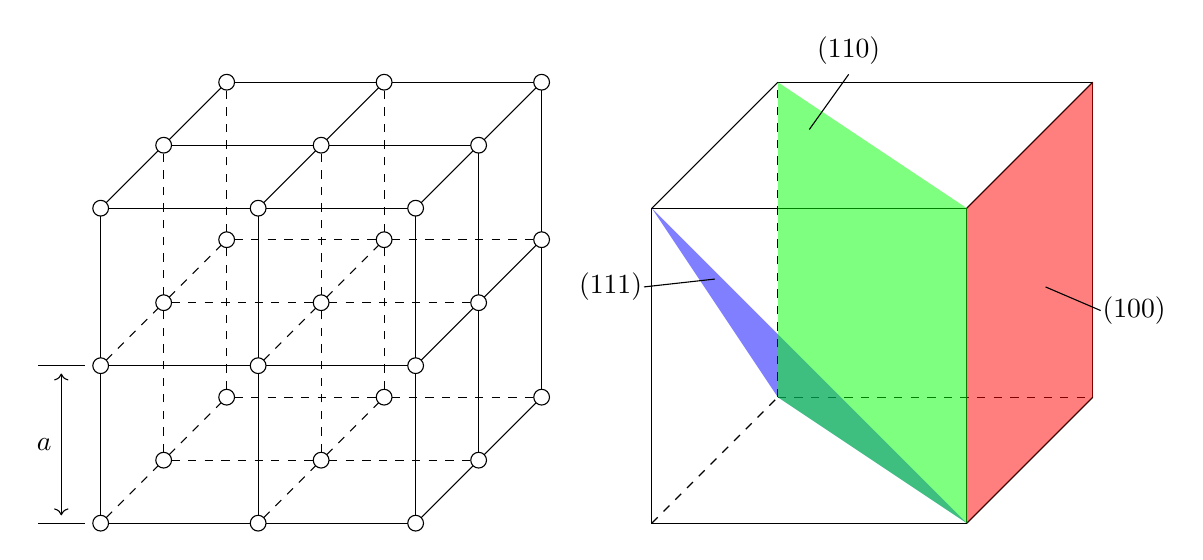
\begin{tikzpicture}
        \draw (0,0) circle [radius=0.1];
        \draw (2,0) circle [radius=0.1];
        \draw (4,0) circle [radius=0.1];
        \draw (4,2) circle [radius=0.1];
        \draw (4,4) circle [radius=0.1];
        \draw (0,2) circle [radius=0.1];
        \draw (0,4) circle [radius=0.1];
        \draw (2,2) circle [radius=0.1];
        \draw (2,4) circle [radius=0.1];
        \draw (0.8,0.8) circle [radius=0.1];
        \draw (0.8,2.8) circle [radius=0.1];
        \draw (0.8,4.8) circle [radius=0.1];
        \draw (2.8,0.8) circle [radius=0.1];
        \draw (4.8,0.8) circle [radius=0.1];
        \draw (2.8,2.8) circle [radius=0.1];
        \draw (2.8,4.8) circle [radius=0.1];
        \draw (4.8,2.8) circle [radius=0.1];
        \draw (4.8,4.8) circle [radius=0.1];				
        \draw (1.6,1.6) circle [radius=0.1];				
        \draw (3.6,1.6) circle [radius=0.1];				
        \draw (5.6,1.6) circle [radius=0.1];				
        \draw (1.6,3.6) circle [radius=0.1];				
        \draw (1.6,5.6) circle [radius=0.1];				
        \draw (3.6,3.6) circle [radius=0.1];				
        \draw (3.6,5.6) circle [radius=0.1];				
        \draw (5.6,3.6) circle [radius=0.1];				
        \draw (5.6,5.6) circle [radius=0.1];
        
        \draw (0.1,0)--(1.9,0);
        \draw (0,0.1)--(0,1.9);
        \draw (0,2.1)--(0,3.9);
        \draw (2.1,0)--(3.9,0);
        \draw (0.1,2)--(1.9,2);
        \draw (0.1,4)--(1.9,4);
        \draw (2.1,2)--(3.9,2);
        \draw (2.1,4)--(3.9,4);
        \draw (2,0.1)--(2,1.9);
        \draw (4,0.1)--(4,1.9);
        \draw (2,2.1)--(2,3.9);
        \draw (4,2.1)--(4,3.9);
        \draw [dashed] (0.8,0.9)--(0.8,2.7);
        \draw [dashed] (2.8,0.9)--(2.8,2.7);
        \draw (4.8,0.9)--(4.8,2.7);
        \draw [dashed] (0.9,0.8)--(2.7,0.8);
        \draw [dashed] (0.9,2.8)--(2.7,2.8);
        \draw (0.9,4.8)--(2.7,4.8);
        \draw [dashed] (0.8,2.9)--(0.8,4.7);
        \draw [dashed] (2.8,2.9)--(2.8,4.7);
        \draw (4.8,2.9)--(4.8,4.7);
        \draw [dashed] (2.9,0.8)--(4.7,0.8);
        \draw [dashed] (2.9,2.8)--(4.7,2.8);
        \draw (2.9,4.8)--(4.7,4.8);
        \draw [dashed] (1.6,1.7)--(1.6,3.5);
        \draw [dashed] (3.6,1.7)--(3.6,3.5);
        \draw (5.6,1.7)--(5.6,3.5);
        \draw [dashed] (1.6,3.7)--(1.6,5.5);
        \draw [dashed] (3.6,3.7)--(3.6,5.5);
        \draw (5.6,3.7)--(5.6,5.5);
        \draw [dashed] (1.7,1.6)--(3.5,1.6);
        \draw [dashed] (1.7,3.6)--(3.5,3.6);
        \draw (1.7,5.6)--(3.5,5.6);
        \draw [dashed] (3.7,1.6)--(5.5,1.6);
        \draw [dashed] (3.7,3.6)--(5.5,3.6);
        \draw (3.7,5.6)--(5.5,5.6);				
        \draw [dashed] (0.07,0.07)--(0.73,0.73);
        \draw [dashed] (0.07,2.07)--(0.73,2.73);
        \draw (0.07,4.07)--(0.73,4.73);				
        \draw [dashed] (2.07,0.07)--(2.73,0.73);
        \draw [dashed] (2.07,2.07)--(2.73,2.73);
        \draw (2.07,4.07)--(2.73,4.73);				
        \draw (4.07,0.07)--(4.73,0.73);
        \draw (4.07,2.07)--(4.73,2.73);
        \draw (4.07,4.07)--(4.73,4.73);				
        \draw [dashed] (0.87,0.87)--(1.53,1.53);
        \draw [dashed] (0.87,2.87)--(1.53,3.53);
        \draw (0.87,4.87)--(1.53,5.53);				
        \draw [dashed] (2.87,0.87)--(3.53,1.53);
        \draw [dashed] (2.87,2.87)--(3.53,3.53);
        \draw (2.87,4.87)--(3.53,5.53);				
        \draw (4.87,0.87)--(5.53,1.53);
        \draw (4.87,2.87)--(5.53,3.53);
        \draw (4.87,4.87)--(5.53,5.53);
        \draw (-0.2,0)--(-0.8,0);				
        \draw (-0.2,2)--(-0.8,2);
        \draw [<->](-0.5,0.1)--(-0.5,1.9);
        \node [left] at(-0.5,1) {$ a $};
        
        \draw (7,0) rectangle (11,4);
        \draw (7,4)--(8.6,5.6);
        \draw (11,4)--(12.6,5.6);
        \draw (8.6,5.6)--(12.6,5.6);
        \draw (11,0)--(12.6,1.6);
        \draw (12.6,1.6)--(12.6,5.6);
        \draw [dashed] (7,0)--(8.6,1.6);
        \draw [dashed] (8.6,1.6)--(8.6,5.6);
        \draw [dashed] (8.6,1.6)--(12.6,1.6);
        \fill [blue,fill opacity=0.5] (8.6,1.6)--(7,4)--(11,0)--(8.6,1.6)--cycle;
        \fill [green,fill opacity=0.5] (8.6,1.6)--(8.6,5.6)--(11,4)--(11,0)--cycle;
        \fill [red,fill opacity=0.5] (11,0)--(12.6,1.6)--(12.6,5.6)--(11,4)--(11,0)--cycle;
        \draw (6.9,3)--(7.8,3.1);
        \node [left] at(7,3) {(111)};
        \draw (9,5)--(9.5,5.7);
        \node [above] at(9.5,5.7) {(110)};
        \draw (12,3)--(12.7,2.7);
        \node [right] at(12.6,2.7) {(100)};
    \end{tikzpicture}
    \caption{立方晶格模型与晶面指数}
    \label{fig-JingGe}
\end{figure}

组成晶体的原子可以看成分别作处在一系列相互平行而且间距一定的平面族上,这些平面称为晶面。在晶面的不同取法中,最重要且最常用的三种即为图\ref{fig-JingGe}\,中的(111)面、(110)面、(100)面,圆括号中的三个数字称为晶面指数。晶面指数的一般取法为:在右手系下取平面在$ x,y,z $轴上的截距$ x_0,y_0,z_0 $,取其倒数之比$ \frac1{x_0}:\frac1{y_0}:\frac1{z_0} $,将其化为最小整数比$ x_1:y_1:z_1 $,则该平面的晶面指数为$ (x_1y_1z_1) $。一般而言,晶面指数为$ (n_1n_2n_3) $的晶面族,其相邻的两个晶面间距$ d=\frac{a}{\sqrt{n_1^2+n_2^2+n_3^2}} $.

\subsubsection{布拉格衍射}

类似光波入射到二维的平面光栅要受到光栅的衍射,电磁波入射到晶体也要受到晶体的衍射。用三维空间中原子组成的格点取代平面上的小孔,可看作是一个三维的光栅网络。晶体对电子波衍射的实质是每个格点上的原子产生的散射波的相干叠加。它们的相干叠加的第一步可看作是统一晶面上各个原子发出的散射波的相干叠加,形成每一个晶面的衍射波;第二步是同一晶面族的不同晶面的衍射波之间的相干叠加。

\begin{figure}[h]
    \centering
    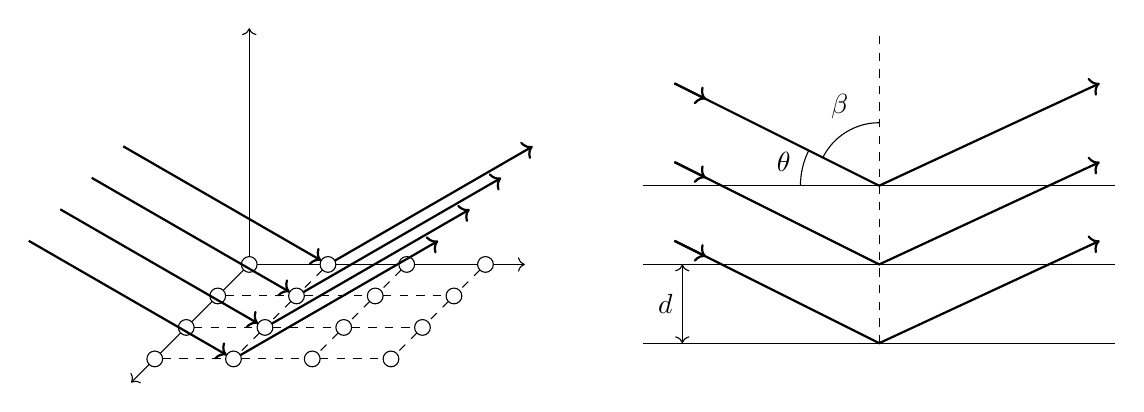
\begin{tikzpicture}
        \draw (-3,0)--(3,0);
        \draw (-3,2)--(3,2);
        \draw (-3,1)--(3,1);
        \draw [dashed] (0,0)--(0,4);
        \draw [<->] (-2.5,0)--(-2.5,1);
        \node [left] at(-2.5,0.5) {$ d $};
        \draw [thick,->] (-2.6,1.3)--(0,0)--(2.8,1.3);
        \draw [thick,->] (-2.6,1.3)--(-2.2,1.1);
        \draw [thick,->] (-2.6,2.3)--(0,1)--(2.8,2.3);
        \draw [thick,->] (-2.6,2.3)--(-2.2,2.1);
        \draw [thick,->] (-2.6,3.3)--(0,2)--(2.8,3.3);
        \draw [thick,->] (-2.6,3.3)--(-2.2,3.1);
        \draw (-1,2) arc (180:154:1);
        \draw (0,2.8) arc (90:154:0.8);
        \node [left] at(-1,2.3) {$\theta$};
        \node at(-0.5,3) {$\beta$};
        
        \draw (-8,1) circle [radius=0.1];
        \draw (-7,1) circle [radius=0.1];
        \draw (-6,1) circle [radius=0.1];
        \draw (-5,1) circle [radius=0.1];
        \draw (-8.4,0.6) circle [radius=0.1];
        \draw (-7.4,0.6) circle [radius=0.1];
        \draw (-6.4,0.6) circle [radius=0.1];
        \draw (-5.4,0.6) circle [radius=0.1];
        \draw (-8.8,0.2) circle [radius=0.1];
        \draw (-7.8,0.2) circle [radius=0.1];
        \draw (-6.8,0.2) circle [radius=0.1];
        \draw (-5.8,0.2) circle [radius=0.1];
        \draw (-9.2,-0.2) circle [radius=0.1];
        \draw (-7.2,-0.2) circle [radius=0.1];
        \draw (-8.2,-0.2) circle [radius=0.1];
        \draw (-6.2,-0.2) circle [radius=0.1];
        \draw [->] (-8,1.1)--(-8,4);
        \draw (-8.07,0.93)--(-8.33,0.67);
        \draw (-8.47,0.53)--(-8.73,0.27);
        \draw (-8.87,0.13)--(-9.13,-0.13);
        \draw [->] (-9.27,-0.27)--(-9.5,-0.5);
        \draw [dashed] (-7.07,0.93)--(-7.33,0.67);
        \draw [dashed] (-7.47,0.53)--(-7.73,0.27);
        \draw [dashed] (-7.87,0.13)--(-8.13,-0.13);
        \draw [dashed] (-6.07,0.93)--(-6.33,0.67);
        \draw [dashed] (-6.47,0.53)--(-6.73,0.27);
        \draw [dashed] (-6.87,0.13)--(-7.13,-0.13);
        \draw [dashed] (-5.07,0.93)--(-5.33,0.67);
        \draw [dashed] (-5.47,0.53)--(-5.73,0.27);
        \draw [dashed] (-5.87,0.13)--(-6.13,-0.13);
        \draw (-7.9,1)--(-7.1,1);
        \draw (-6.9,1)--(-6.1,1);
        \draw (-5.9,1)--(-5.1,1);
        \draw [->] (-4.9,1)--(-4.5,1);
        \draw [dashed] (-8.3,0.6)--(-7.5,0.6);
        \draw [dashed] (-7.3,0.6)--(-6.5,0.6);
        \draw [dashed] (-6.3,0.6)--(-5.5,0.6);
        \draw [dashed] (-8.7,0.2)--(-7.9,0.2);
        \draw [dashed] (-7.7,0.2)--(-6.9,0.2);
        \draw [dashed] (-6.7,0.2)--(-5.9,0.2);
        \draw [dashed] (-9.1,-0.2)--(-8.3,-0.2);
        \draw [dashed] (-8.1,-0.2)--(-7.3,-0.2);
        \draw [dashed] (-7.1,-0.2)--(-6.3,-0.2);
        \draw [thick,->] (-9.60,2.5)--(-7.086,1.05);
        \draw [thick,->] (-10.0,2.1)--(-7.486,0.65);
        \draw [thick,->] (-10.40,1.7)--(-7.886,0.25);
        \draw [thick,->] (-10.80,1.3)--(-8.286,-0.15);
        \draw [thick,->] (-6.91,1.05)--(-4.40,2.5);
        \draw [thick,->] (-7.31,0.65)--(-4.80,2.1);
        \draw [thick,->] (-7.71,0.25)--(-5.20,1.7);
        \draw [thick,->] (-8.11,-0.15)--(-5.60,1.3);
    \end{tikzpicture}
    \caption{同一晶面与不同晶面的散射波示意图}
    \label{fig-scatt}
\end{figure}

处在同一平面上的原子组成一个晶面,它们的散射波相干叠加的结果遵从反射定律。而从间隔为$ d $的相邻两个晶面反射的两束波的程差为$ 2d\sin\theta $,$ \theta $为入射角与晶面的夹角。显然只有满足
\[2d\sin\theta=k\lambda,\qquad k=1,2,3,\cdots\]
才能形成干涉极大。上式称为晶体衍射的布拉格条件,如果改用常用的入射角$ \beta $表示,则布拉格条件可改写为
\[2d\cos\beta=k\lambda,\qquad k=1,2,3,\cdots\]
在本次实验中,已知晶面间距$ d $,通过测量衍射极大时的入射角$ \beta $以求得波长$\lambda$.

由于不同晶面族的曲线不同,晶面间隔也不同,因此当入射波方向及波长固定、晶体取向固定时,不同取向的晶面不能同时满足布拉格条件,甚至没有一族晶面能够满足布拉格条件。为了观察到尽可能多的衍射极大,得到尽可能多的关于晶体结构的信息,在研究晶体结构的实际工作中,采用不同的方法:转动晶体、采用多晶或粉末样品代替单晶、采用包含波长连续变化的X射线代替单一波长的X射线。在本实验中使用入射方向固定、波长单一的微波及单晶模型,从而采用转动晶体模型和接收喇叭的方向来进行对不同晶面的研究。


\section{实验内容}
实验中所用微波频率一致,均为9.4\,GHz,打开电源后将微波频率设置为9.4\,GHz,并调整实验仪器在桌面上的位置与角度,使得检波器扫描范围能达到$ \pm50^\circ $。

\subsection{$^*$实验 1 :微波的单缝衍射}
此小节为选做实验。


转动接收臂使其指针指向载物台的$ 0^\circ $刻线,打开振荡器的电源,转动载物台,使其上的$ 180^\circ $刻线与发射臂的指针一致,调节发生器与接受器姿态,使其正对,微调接收喇叭的朝向,使得在$ \pm20^\circ $处的差异在2\,mV以内。

调节衰减器,使二者正对时接收电表的指示在150\,mV左右。

仪器安装时,按需要先调整单缝衍射板的缝宽,然后把单缝衍射板放到载物台,并使狭缝所在平面与入射方向垂直(微调狭缝角度使得当正对发生器的接收电表示数极大),把单缝的底座固定在载物台上。

转动接收臂,在$ -40^\circ\sim40^\circ $内每隔$ 2^\circ $记下一次接收信号的大小。

为了准确测量波长,需仔细寻找衍射极小的位置。在衍射极小附近,以$ 1^\circ $为步长精扫接收信号的变化。可把衰减器向零处旋转,以增大发射信号的强度,进而提高测量的灵敏度。

根据记录数据,画出单缝衍射强度与衍射角度的关系曲线。并根据微波衍射强度一级极小角度$ \varphi $和缝宽$a$,计算微波波长$\lambda$和其百分误差。

\subsection{实验 2 :微波的双缝干涉}
放置双缝前,与实验1一样进行实验仪对准确认,使得发生器、接收器分别于$ 180^\circ,0^\circ $处正对,接收信号在$ \pm20^\circ $处强度相当。调节微波发射功率使得在零级极大处接收信号强度在150\,mV左右。

按要求调整双缝干涉板的缝宽均为3.5\,cm。将双缝缝干射板安置在支座上时,应使双缝板平面与载物圆台上$ 90^\circ $指示线一致。在$ -50^\circ\sim50^\circ $范围内,每改变$ 2^\circ $读取一次液晶显示器的读数,并记录下来,然后就可以画出双缝干涉强度与角度的关系曲线。

在两侧零级极大、零级极小、一级极小处以$ 1^\circ $为步长进行精扫,绘制精扫结果图象以确定极值点。

根据微波干涉强度零级极大、零级极小、一级极大角度和缝宽$a$、缝间间隔$ b $,计算微波波长$\lambda$和其百分误差。

\subsection{实验 3 :迈克尔逊干涉实验}
根据微波的前进方向设置迈克尔逊干涉仪,在极大位置适当调节微波发生功率使其大于100\,mV,便于观察接收信号强度的变化与极小值。将可移动反射板装在一旋转读数机构上后,然后移动旋转读数机构上的手柄,使得可移动反射板移动,测出$ n+1 $个微波极小值,并同时从读数机构上读出可移反射板的移动距离$ L $,则波长满足$ \lambda=\frac{2L}{n} $。

\subsection{实验 4 :布拉格衍射}
同之前的实验一样,实验开始前需检查发生器和检波器的正对情况。
\subsubsection{ 100 晶面}
将发生器与检波器正对,调节微波发生功率使得接收信号为$ 150\,\mathrm{mV} $左右。安装模型晶体,转动载物圆盘使得发生器位于$ -30^\circ $(即$ 330^\circ $)处,转动接收器使其位于$ 30^\circ $处,即使得入射角与探测方向相对晶面法线对称。将入射角在$ 30^\circ\sim80^\circ $范围内以$ 2^\circ $为步长步进,在相应的探测位置读得并记录接收信号强度。绘制入射角与接收信号强度间的图象。

在信号强度极大值点附近以$ 1^\circ $为步长进行精扫,以确定极大值点对应的入射角。进而求得微波波长$ \lambda=2d\cos\beta $并计算百分误差。

\subsubsection{ 110 晶面}
大致步骤与 100 晶面时一致,不同在于 100 晶面的晶面法线方向为载物圆盘上$ 0^\circ $方向,而 110 晶面的晶面法线方向为载物圆盘上$ 45^\circ $方向。此外粗扫时入射角范围调整为$ 30^\circ\sim70^\circ $,精扫时由于接收信号较弱可适当调节微波发生功率。

\section{实验结果与数据处理}

\noindent\textbf{实验条件确认:}
本次实验采用的微波条件为:
\begin{table}[H]\centering
    %\renewcommand{\arraystretch}{1.5} % 调整行间距为 1.5 倍
    %\setlength{\tabcolsep}{1.5mm} % 调整列间距
    \begin{tabular}{cccccccccc}\toprule
        频率 & 波长  \\
        \midrule
        $9.4 \ \mathrm{GHz}$ & $3.1892 \ \mathrm{cm}$ \\
        \bottomrule
    \end{tabular}
\end{table}
根据微波发生器侧面的列表,旋转“频率调节”按钮,使发生器输出频率为 $9.4 \ \mathrm{GHz}$ 的微波。

对角度的规定,我们采用数学通用规范,即以顺时针方向为负角度,逆时针方向为正角度。

实验过程中,为了尽量减小误差,每次子实验前都需要微波仪器进行对准确认。分别在在正负 20° 处观察接收器的电压值,反复微调接收器角度,使得两点测量到信号强度的差的绝对值不超过 0.2 mV 。对准结果如下表所示:
\begin{table}[H]\centering
    %\renewcommand{\arraystretch}{1.5} % 调整行间距为 1.5 倍
    %\setlength{\tabcolsep}{1.5mm} % 调整列间距
    \caption{微波仪器对准结果}
    \label{微波仪器对准结果}
    \begin{tabular}{ccccc}
        \toprule
            子实验名称 & $+20^\circ$ & $0^\circ$ & $-20^\circ$ & 信号差 (mV) \\
            \midrule
            单缝衍射 & 21.2 & 189.2 & 21.3 & -0.1 \\ 
            双缝干涉 & 11.0 & 158.3 & 11.2 & -0.2 \\ 
            迈克尔逊干涉 & 10.7 & 141.7 & 10.6 & +0.1 \\ 
            布拉格(100 晶面) & 11.5 & 162.7 & 11.4 & +0.1 \\ 
            布拉格(110 晶面) & 11.2 & 161.9 & 11.4 & -0.2 \\ 
            \bottomrule
        \end{tabular}
\end{table}

为了最大限度地利用已知数据,同时又尽可能地降低二次误差,需要取角度的极值时,我们会先对原数据进行适当的拟合,然后再求极值的数值解。拟合的方法因子实验和数据而异,我们不再报告中详细赘述。另外,为保证阅读的流畅性,具体的实验数据列表会尽量放在每一小节(子实验)的最后,以强调更为重要的实验结果。

\begin{graybox}
    $^*$ 按老师的要求,本次实验的全部数据图均需手绘,但考虑到作图的美观性和准确性,我们在给出手绘图的同时,也会给出部分用 Matlab 所作的数据图,以方便进一步的分析。
\end{graybox}


\subsection{$^*$实验 1 :微波的单缝衍射}
按老师的要求,此实验为选做实验,我们仅对测的数据进行一些简单的分析和对比,并不由此求解所测得的波长。

单缝缝宽 $b = 8 \ \mathrm{cm}$,测得的实验数据如表 \ref{} 所示。作出接收器电压值 $U$ (正比于辐照度 $I$) 关于角度 $\theta$ 的变化情况,如图 \ref{单缝衍射实验数据} 所示。

\begin{figure}[H]\centering
\begin{subfigure}[b]{0.33\columnwidth}\centering
    \includegraphics[height=150pt]{assets/1 单缝/1 单缝.png}
    \caption{单缝衍射粗扫}
\end{subfigure}
\begin{subfigure}[b]{0.33\columnwidth}\centering
    \includegraphics[height=150pt]{assets/1 单缝/1 单缝 极小 -.jpg}
    \caption{负方向第一个极小值}
\end{subfigure}\hfill
\begin{subfigure}[b]{0.33\columnwidth}\centering
    \includegraphics[height=150pt]{assets/1 单缝/1 单缝 极小 +.jpg}
    \caption{正方向第一个极小值}
\end{subfigure}
\caption{单缝衍射}
\label{单缝衍射}
\end{figure}

正负方向上的极小值读数分别为 $\theta_{0, +} = 23.43^\circ $ 和 $\theta_{0, -} = 22.76^\circ $。为了降低仪器角偏移对测量结果的影响,取正负方向两个极小值的对应角度的算术平均,得到极小值对应的角度为 $\theta_0 = 23.095^\circ = 0.4031 \ \mathrm{rad}$。代入公式 $b \sin \theta_0 = \lambda$,计算出实验波长值,与理论波长 $\lambda = 3.1892 \ \mathrm{cm}$ 作对比,并由公式 $\eta  = \frac{\lambda_{\text{exp}} - \lambda_{\text{theo}}}{\lambda_{\text{theo}}}\times 100\, \%$ 求得两者的相对误差(含正负的相对误差),最终得到:
\begin{equation}\boldmath
    \lambda_{\text{exp}} = 3.1381 \ \mathrm{cm},\quad \eta = - 1.6037\, \%
\end{equation}
其中 $\lambda_{\text{theo}}$ 为理论波长,在本次实验是 $\lambda_{\text{theo}} = 3.1892 \ \mathrm{cm}$,$\lambda_{\text{exp}}$ 为实验测得的波长。





不妨再将电压的实验数据点与理论值作对比。在同一坐标系下,同时作出辐照度(正比于电压 $U$)的理论变化曲线与实际测得的数据点,如图 \ref{单缝对比} 所示,其中理论值的最大电压取了 190 mV。
\begin{figure}[H]\centering
    \includegraphics[width=\columnwidth]{assets/1 单缝/单缝 对比.pdf}
    \caption{单缝衍射理论值与实验值对比}\label{单缝对比}
\end{figure}
由图可以看到,实验值大致符合理论预测,但在一些细节上仍有差别。其一是 $\left| \theta \right| $ 较大时,辐照度的“回升”不明显(相比理论值);其二是在 $\theta \in (-10^\circ, -1^\circ)$ 的范围内,实验值有明显降低,这很可能是因为实验台两侧环境不对称,$\theta < 0$ 一侧空旷,而 $\theta > 0$ 一侧有隔板。


\begin{center}
\noindent\begin{minipage}{0.65\columnwidth}
\begin{table}[H]\centering
    %\renewcommand{\arraystretch}{1.5} % 调整行间距为 1.5 倍
    %\setlength{\tabcolsep}{1.5mm} % 调整列间距
    \caption{单缝衍射实验数据}
    \label{单缝衍射实验数据}
    \begin{tabular}{cccccc}\toprule
        $\theta \ \mathrm{(^\circ)}$  & $U_{\theta+}$ (mV) & $U_{\theta-}$ (mV) & $\theta \ \mathrm{(^\circ)}$  & $U_{\theta+}$ (mV) & $U_{\theta-}$ (mV) \\
        \midrule
        0	&189.2	&189.2 & 22	&0.1	&0.0 \\
        2	&175	&170   & 24	&0	    &0.0 \\
        4	&163.8	&120.6 & 26	&0.1	&0.0 \\
        5	&157.5	&107.6 & 28	&0.2	&0.1 \\
        6	&147.9	&108.5 & 30	&0.3	&0.9 \\
        7	&131.6	&112.9 & 32	&1.3	&2.9 \\
        8	&112.3	&112.0 & 34	&2.2	&2.3 \\
        9	&93.7	&107.4 & 36	&2	    &0.3 \\
        10	&77.5	&94.1  & 38	&0.5	&0.0 \\
        12	&57.4	&48.3  & 40	&0.2	&1.7 \\
        14	&42.5	&24.9  & 42	&1.0	&4.7 \\
        16	&28.1	&10.3  & 44	&1.3	&1.7 \\
        18	&10.8	&3.0   & 45	&0.8	&0.3 \\
        20	&1.1	&0.2   &    &       &    \\
        \bottomrule
    \end{tabular}
\end{table}
\end{minipage}\hfill\begin{minipage}{0.35\columnwidth}
    \begin{table}[H]\centering
        %\renewcommand{\arraystretch}{1.5} % 调整行间距为 1.5 倍
        %\setlength{\tabcolsep}{1.5mm} % 调整列间距
        \caption{单缝衍射极小值附近数据}
        \label{单缝衍射极小值附近数据}
    \begin{tabular}{ccc}\toprule
        $\theta \ \mathrm{(^\circ)}$ & $U_{\theta+}$ (mV) & $U_{\theta-}$ (mV) \\ 
        \midrule
        20	&3.8	&1.0 \\
        21	&0.9	&0.2 \\
        22	&0.2	&0.0 \\
        23	&0.0	&0.0 \\
        24	&0.0	&0.1 \\
        25	&0.2	&0.0 \\
        26	&0.4	&0.0 \\
        27	&0.5	&0.0 \\
        28	&0.6	&0.1 \\
        \bottomrule
    \end{tabular}
    \end{table}
\end{minipage}\end{center}


\subsection{实验 2 :微波的双缝干涉}
两条双缝的缝宽为 $b = 3.5 \ \mathrm{cm}$,狭缝中心的距离为 $a = 3.5 + 5 = 8.5 \ \mathrm{cm}$。实验测得的数据如表 \ref{双缝衍射粗扫数据} 至 表 \ref{双缝衍射 1 级极小} 所示。


\begin{table}[H]\centering
    %\renewcommand{\arraystretch}{1.5} % 调整行间距为 1.5 倍
    %\setlength{\tabcolsep}{1.5mm} % 调整列间距
    \caption{双缝衍射粗扫数据}
    \label{双缝衍射粗扫数据}
\begin{tabular}{cccccccccc}\toprule
    $\theta \ \mathrm{(^\circ)}$  & $U_{\theta+}$ (mV) & $U_{\theta-}$ (mV) & $\theta \ \mathrm{(^\circ)}$  & $U_{\theta+}$ (mV) & $U_{\theta-}$ (mV) \\
    \midrule
    0	&142.8	&142.8 &26	&71.3	&32.5   \\
    2	&138.4	&126.8 &28	&28	    &8.9    \\
    4	&116.3	&97.5  &30	&7.5	&4.7    \\
    6	&64.6	&38.2  &32	&3.4	&5.1    \\
    8	&12.3	&1.5   &34	&3.6	&9.5    \\
    10	&0.6	&0.4   &36	&5.5	&16.2   \\
    12	&0.2	&3.3   &38	&11.8	&14.1   \\
    14	&5.7	&17.4  &40	&11.6	&5      \\
    16	&29.2	&46.3  &42	&4.8	&3.1    \\
    18	&54.5	&81.5  &44	&3.6	&16.1   \\
    20	&81.6	&99    &46	&16.4	&40.3   \\
    22	&100.2	&93.6  &48	&35.3	&25.9   \\
    24	&98	    &60.4  &50	&28.4	&3.4    \\
    \bottomrule
\end{tabular}
\end{table}


\begin{center}
\noindent\begin{minipage}{0.35\columnwidth}
    \begin{table}[H]\centering
        %\renewcommand{\arraystretch}{1.5} % 调整行间距为 1.5 倍
        %\setlength{\tabcolsep}{1.5mm} % 调整列间距
        \caption{双缝衍射 0 级极小}
        \label{双缝衍射 0 级极小}
        \resizebox{0.93\columnwidth}{!}{
    \begin{tabular}{cccc}\toprule
        $\theta \ \mathrm{(^\circ)}$ & $U_{\theta+}$ (mV) & $\theta \ \mathrm{(^\circ)}$ & $U_{\theta-}$ (mV) \\ 
        \midrule
        8	&13.8	&6	&39.2   \\
        9	&2.4	&7	&11.2   \\
        10	&0.7	&8	&2.2    \\
        11	&0.0	&9	&0.3    \\
        12	&0.2	&10	&0.3    \\
        13	&1.4	&11	&1.3    \\
        14	&8.8	&12	&3.8    \\
        15	&19.0	&13	&8.9    \\
        16	&29.2	&14	&18.1   \\      
        \bottomrule
    \end{tabular}
    }
    \end{table}
\end{minipage}\hfill
\begin{minipage}{0.29\columnwidth}
\begin{table}[H]\centering
    %\renewcommand{\arraystretch}{1.5} % 调整行间距为 1.5 倍
    %\setlength{\tabcolsep}{1.5mm} % 调整列间距
    \caption{双缝衍射 1 级极大}
    \label{双缝衍射 1 级极大}
    \resizebox{\columnwidth}{!}{
        \begin{tabular}{cccc}\toprule
            $\theta \ \mathrm{(^\circ)}$ & $U_{\theta+}$ (mV)  & $U_{\theta-}$ (mV) \\ 
            \midrule
            18	&59.1	&80.5   \\
            19	&70.5	&91.7   \\
            20	&78.6	&100.2  \\
            21	&89.4	&100.9  \\
            22	&100.5	&92.2   \\
            23	&99.8	&76.5   \\
            24	&96.5	&62.3   \\
            25	&84.3	&49.9   \\
            \bottomrule
        \end{tabular}
    }
\end{table}
\end{minipage}
\begin{minipage}{0.35\columnwidth}
    \begin{table}[H]\centering
        %\renewcommand{\arraystretch}{1.5} % 调整行间距为 1.5 倍
        %\setlength{\tabcolsep}{1.5mm} % 调整列间距
        \caption{双缝衍射 1 级极小}
        \label{双缝衍射 1 级极小}
        \resizebox{0.93\columnwidth}{!}{
        \begin{tabular}{cccc}\toprule
            $\theta \ \mathrm{(^\circ)}$ & $U_{\theta+}$ (mV)  & $\theta \ \mathrm{(^\circ)}$ & $U_{\theta-}$ (mV) \\ 
            \midrule
            30	&7.0	&28	&17.8   \\
            31	&4.1	&29	&7.5    \\
            32	&2.4	&30	&5.3    \\
            33	&2.2	&31	&4.5    \\
            34	&2.9	&32	&4.3    \\
            35	&3.5	&33	&6.9    \\
            36	&4.9	&34	&9.4    \\
            37	&8.7	&35	&13.0   \\
            38	&12.6	&36	&15.9   \\
            \bottomrule
        \end{tabular}
        }
    \end{table}
\end{minipage}
\end{center}

根据上面数据作出电压 $U$ 关于角度 $\theta$ 的变化情况,如图 \ref{} 所示。
再作出极值点附近的辐照度变化情况,如图 \ref{}。然后据图对极值所在角度进行读数,依据公式 (\ref{}) 计算出波长的实验值,并求出相对误差 $\eta $。
\begin{equation} 
\text{极大值:} a \sin \theta = m \lambda,\quad \text{极小值:} a \sin \theta = \left(m + \frac{1}{2}\right) \lambda
\end{equation}
注意上式中的 $a$ 是指两条狭缝的中心距离,也即 $a = 3.5 \ \mathrm{cm} + 5 \ \mathrm{cm}  = 8.5\ \mathrm{cm}$。计算结果如下表所示:
\begin{table}[H]\centering
    %\renewcommand{\arraystretch}{1.5} % 调整行间距为 1.5 倍
    %\setlength{\tabcolsep}{1.5mm} % 调整列间距
    \caption{双缝衍射波长测量结果}
    \label{双缝衍射波长测量结果}
\begin{tabular}{cccccccccc}\toprule
    项目 & $\theta_+$ & $\theta_-$ & $\bar{\theta}$ & Formula & $\boldmath \lambda_{\text{exp}}$  & $\boldmath \eta$ \\
    \midrule
    0 级极小 & $11.43^\circ$ &  $9.58^\circ$  & $10.505^\circ$ & $a \sin \theta = 0.5\,\lambda$ & \textbf{3.0995 cm} &  \textbf{- 2.8138 \,\%}\\
    1 级极大 & $22.39^\circ$ &  $20.58^\circ$ & $21.485^\circ$ & $a \sin \theta = \lambda$      & \textbf{3.1132 cm} &  \textbf{- 2.3834 \,\%}\\
    1 级极小 & $32.41^\circ$ &  $31.60^\circ$ & $32.005^\circ$ & $a \sin \theta = 1.5\,\lambda$ & \textbf{3.0033 cm} &  \textbf{- 5.8292 \,\%}\\
    \bottomrule
\end{tabular}
\end{table}


\begin{figure}[H]\centering
\begin{subfigure}[b]{0.5\columnwidth}\centering
    \includegraphics[height=170pt]{assets/2 双缝/2 双缝 粗扫.png}
    \vspace*{7mm}
    \caption{手绘图}
\end{subfigure}\hfill
\begin{subfigure}[b]{0.5\columnwidth}\centering
    \includegraphics[height=180pt]{assets/2 双缝/2 双缝 粗扫.pdf}
    \caption{Matlab 绘图}
\end{subfigure}
\caption{双缝干涉粗扫数据}
\end{figure}



\begin{figure}[H]\centering
\begin{subfigure}[b]{0.5\columnwidth}\centering
    \includegraphics[height=132pt]{assets/2 双缝/双 0小+.png}
    \caption{0 级极小 (正方向)}
\end{subfigure}\hfill
\begin{subfigure}[b]{0.5\columnwidth}\centering
    \includegraphics[height=132pt]{assets/2 双缝/双 0小-.png}
    \caption{0 级极小 (负方向)}
\end{subfigure}
\begin{subfigure}[b]{0.5\columnwidth}\centering
    \includegraphics[height=132pt]{assets/2 双缝/双 1大+.png}
    \caption{1 级极大 (正方向)}
\end{subfigure}\hfill
\begin{subfigure}[b]{0.5\columnwidth}\centering
    \includegraphics[height=132pt]{assets/2 双缝/双 1大-.png}
    \caption{1 级极大 (负方向)}
\end{subfigure}
\begin{subfigure}[b]{0.5\columnwidth}\centering
    \includegraphics[height=132pt]{assets/2 双缝/双 1小+.png}
    \caption{1 级极小 (正方向)}
\end{subfigure}\hfill
\begin{subfigure}[b]{0.5\columnwidth}\centering
    \includegraphics[height=132pt]{assets/2 双缝/双 1小-.png}
    \caption{1 级极小 (正方向)}
\end{subfigure}
\caption{双缝干涉极值细扫数据}
\end{figure}

取三个极值对应波长实验值的算术平均,得到最终测量结果:
\begin{equation}\boldmath
    \lambda_{\text{exp}} = 3.0720 \ \mathrm{cm},\quad \eta = - 3.6754\, \%
\end{equation}

同样,我们将电压的实验数据与理论值作对比。依据实验条件,令波长 $\lambda = 3.1892$,狭缝中心距离 $a = 8.5 \ \mathrm{cm}$,缝宽 $b = 3.5 \ \mathrm{cm}$。由公式 $I = I(0)\sinc^2 \beta \cos \alpha $,在同一坐标系下,作出理论值与实际数据点的图像,如下:
\begin{figure}[H]\centering
\includegraphics[width=\columnwidth]{assets/2 双缝/双缝 对比.pdf}
\caption{双缝干涉理论值与实验值对比}\label{双缝干涉理论值与实验值对比}
\end{figure}

从图中可以看到,一方面,实验测得的数据整体向正方向发生了 $1^\circ$ 左右的偏移,这也可能是实验台两侧环境不对称导致的,还可能与实验前的对准不够精确有关。另一方面,在 $\left| \theta \right| $ 较大时,实验值与理论值的差距较大,甚至连峰和谷出现的趋势都不同,这可能是因为由发生器产生的微波穿过双缝时,不能够视为理想的均匀线光源。至于更具体的原因,有待进一步的研究。



\subsection{实验 3 :迈克尔逊干涉实验}
如图 \ref{} 搭建实验装置,测得的最小点读数为:
\begin{table}[H]\centering
    %\renewcommand{\arraystretch}{1.5} % 调整行间距为 1.5 倍
    %\setlength{\tabcolsep}{1.5mm} % 调整列间距
    \caption{}
    \label{}
\begin{tabular}{cccccccccc}\toprule
    最小点位置 & 0.95 cm & 2.57 cm & 4.22 cm & 5.59 cm \\
    \bottomrule
\end{tabular}
\end{table}
用函数 $x = kn + b$ 对原数据进行最小二乘的线性拟合,其中 $n$ 为数据点的序号,$x$ 为最小点的位置读数(单位是 $\ \mathrm{cm}$),可以得到:
\begin{gather}
x = 1.5575\, n - 0.56 \\ 
\text{SSE} = 0.02043,\  R^2 = 0.9983,\ R^2_\text{adj} = 0.9975,\   \text{RMSE} = 0.1011
\end{gather}
由图 \ref{迈克尔逊干涉实验结果拟合} 和几个拟合优度参数可以看到,拟合效果非常不错,可信度较高。根据拟合结果计算波长的实验值,并求与理论波长的相对误差:
\begin{equation}\boldmath
    \lambda_{\text{exp}} = 2 \frac{\Delta x}{\Delta n} = 3.1150 \ \mathrm{cm},\quad \eta = - 2.3266 \,\%
\end{equation}
\begin{figure}[H]\centering
    \includegraphics[width=\columnwidth]{assets/3 迈克尔/2024-11-02_17-05-08.pdf}
    \caption{迈克尔逊干涉实验结果拟合}\label{迈克尔逊干涉实验结果拟合}
\end{figure}


\subsection{实验 4 :布拉格衍射}
\subsubsection{ 100 晶面}
实验数据如表 \ref{100 晶面粗扫数据} 所示,据此作出相应的图像,如图 \ref{100} 所示。

\begin{figure}[H]\centering
\begin{subfigure}[b]{0.5\columnwidth}\centering
    \includegraphics[height=220pt]{assets/4 布拉格/布 100.png}
    \caption{100 晶面粗扫}
\end{subfigure}\hfill
\begin{subfigure}[b]{0.5\columnwidth}\centering
    \includegraphics[height=220pt]{assets/4 布拉格/布 100大.png}
    \caption{100 镜面细扫}
\end{subfigure}
\caption{布拉格衍射 (100 晶面) 实验数据}
\label{100}
\end{figure}

\begin{center}
\noindent\begin{minipage}{0.65\columnwidth}
\begin{table}[H]\centering
    %\renewcommand{\arraystretch}{1.5} % 调整行间距为 1.5 倍
    %\setlength{\tabcolsep}{1.5mm} % 调整列间距
    \caption{100 晶面粗扫数据}
    \label{100 晶面粗扫数据}
    \begin{tabular}{cccccc}\toprule
        $\theta \ \mathrm{(^\circ)}$ & $U_{\theta+}$ (mV) & $\theta \ \mathrm{(^\circ)}$ & $U_{\theta-}$ (mV) & $\theta \ \mathrm{(^\circ)}$ & $U_{\theta+}$ (mV) \\ 
        \midrule
        30	&2.8	&48	&4.1	&66	&81.7   \\
        32	&3.1	&50	&8.6	&68	&117.8  \\
        34	&2.4	&52	&1.5	&70	&66.6   \\
        36	&2.6	&54	&1.3	&72	&8.5    \\
        38	&2.8	&56	&3.8	&74	&10.6   \\
        40	&4.9	&58	&4.6	&76	&23.7   \\
        42	&3.1	&60	&11.7   &78	&0.0    \\
        44	&0.5	&62	&30.0   &80	&9.2    \\
        46	&0.5	&64	&31.0   &	&       \\
        \bottomrule
    \end{tabular}
\end{table}
\end{minipage}\hfill\begin{minipage}{0.32\columnwidth}
\begin{table}[H]\centering
    %\renewcommand{\arraystretch}{1.5} % 调整行间距为 1.5 倍
    %\setlength{\tabcolsep}{1.5mm} % 调整列间距
    \caption{100 晶面细扫数据}
    \label{100 晶面细扫数据}
    \begin{tabular}{cc}\toprule
        $\theta \ \mathrm{(^\circ)}$ & $U_{\theta+}$ (mV) \\ 
        \midrule
        64&	31.5    \\
        65&	60.3    \\
        66&	86.1    \\
        67&	99.4    \\
        68&	115.4   \\
        69&	107.3   \\
        70&	46.6    \\
        71&	7.8     \\
        72&	9       \\  
        \bottomrule
    \end{tabular}
\end{table}
\end{minipage}\end{center}

从图中可读数极大值对应角度约为 $\beta = 68.62^\circ$ ,100 晶面对应的面间距为 $d = 4 \ \mathrm{cm}$,代入公式计算出波长的实验值:
\begin{equation}\boldmath
    \lambda_\text{exp} = 2d \cos \beta = 2.9164 \ \mathrm{cm},\quad 
    \eta = -8.5534 \,\%
\end{equation}

\subsubsection{110 晶面}
实验数据如表 \ref{} 所示,据此作出相应的图像,如图 \ref{} 所示。
\begin{figure}[H]\centering
\begin{subfigure}[b]{0.5\columnwidth}\centering
    \includegraphics[height=220pt]{assets/4 布拉格/布 110.png}
    \caption{110 晶面粗扫}
\end{subfigure}\hfill
\begin{subfigure}[b]{0.5\columnwidth}\centering
    \includegraphics[height=220pt]{assets/4 布拉格/布 110大.png}
    \caption{110 晶面细扫}
\end{subfigure}
\caption{布拉格衍射 (110 晶面) 实验数据}
\label{110}
\end{figure}

从图中可读数极大值对应角度约为 $\beta = 54.43^\circ$ ,110 晶面对应的面间距为 $d = 2\sqrt{2} \ \mathrm{cm}$,由此计算出波长的实验值:
\begin{equation}\boldmath
    \lambda_\text{exp} = 2d \cos \beta = 3.2906 \ \mathrm{cm},\quad \eta = + 3.1787 \,\%
\end{equation}

\begin{center}
\noindent\begin{minipage}{0.65\columnwidth}
\begin{table}[H]\centering
    %\renewcommand{\arraystretch}{1.5} % 调整行间距为 1.5 倍
    %\setlength{\tabcolsep}{1.5mm} % 调整列间距
    \caption{110 晶面粗扫数据}
    \label{110 晶面粗扫数据}
    \begin{tabular}{cccccc}\toprule
        $\theta \ \mathrm{(^\circ)}$ & $U_{\theta+}$ (mV) & $\theta \ \mathrm{(^\circ)}$ & $U_{\theta-}$ (mV) & $\theta \ \mathrm{(^\circ)}$ & $U_{\theta+}$ (mV) \\ 
        \midrule
        30	&0.1	&48	&4.8	&66	&2.9    \\
        32	&0.1	&50	&8.4	&68	&0.0    \\
        34	&0.2	&52	&41.6	&70	&0.1    \\
        36	&0.6	&54	&81.8	&	&       \\
        38	&0.5	&56	&63.6	&	&       \\
        40	&1.2	&58	&36.8	&	&       \\
        42	&1.6	&60	&34.7	&	&       \\
        44	&2.4	&62	&2.3	&	&       \\
        46	&5.2	&64	&2.2	&	&       \\    
        \bottomrule
    \end{tabular}
\end{table}
\end{minipage}\hfill\begin{minipage}{0.32\columnwidth}
\begin{table}[H]\centering
    %\renewcommand{\arraystretch}{1.5} % 调整行间距为 1.5 倍
    %\setlength{\tabcolsep}{1.5mm} % 调整列间距
    \caption{110 晶面细扫数据}
    \label{110 晶面细扫数据}
    \begin{tabular}{cc}\toprule
        $\theta \ \mathrm{(^\circ)}$ & $U_{\theta+}$ (mV) \\ 
        \midrule
        51&	24.0    \\
        52&	45.3    \\
        53&	64.4    \\
        54&	82      \\
        55&	91.5    \\
        56&	66.7    \\
        57&	51.3    \\
        58&	39.3    \\
        59&	32.7    \\       
        \bottomrule
    \end{tabular}
\end{table}
\end{minipage}\end{center}

\section{思考题}

\subsection*{6.1 各实验内容主要误差影响是什么?}

无论哪个子实验,都受到实验环境的干扰,以及微波实验仪本身的局限性限制。

对于前者,实验环境的封闭性和对称性都不好:一边有吸波墙的隔绝,而另一边则面向实验者,相对比较空旷。这样的环境不利于微波的传播,也容易受到外界干扰。另外,部分实验仪器的安装也不够稳固,导致实验者在调整时很难保证实验仪器的平衡和稳定。

对于后者,一方面是试验仪上两个喇叭的对正关系不好调整,且受限于实验环境的不对称,理论上不可能调整到真实的正对关系。微波与单缝、双缝、反射板是否正交几乎只能靠目测调节,人为主观判断的因素较多。另一方面,微波接收器的示数极不稳定,这为实验数据的准确读取带来了很大的困难。

并且,不得不考虑的是,微波波长约为 $3 \ \mathrm{cm}$,这与实验室中许多物品的尺度接近,容易发生复杂的、相互耦合的干涉衍射现象,影响实验结果的准确性。

\noindent 对每个子实验,具体的误差来源如下:
\begin{enumerate}
\item 单缝衍射:单缝反射板并不一定完全垂直,可能存在一定角度;单缝的缝宽可能不均匀或不准确,导致衍射效果存在误差。
\item 双缝干涉:双缝的缝宽可能不均匀或不准确,导致干涉效果存在误差;双缝的中心距离可能不准确,双缝板与发射喇叭、接受喇叭的角度也会影响辐照度的测量结果。
\item 迈克尔逊干涉:两个反射板不一定完全垂直,可能存在一定角度,同时分光板也不一定恰好处于 $45^\circ$ 处;反射板的平行度可能不够好;反射板的平移可能不均匀。
\item 布拉格衍射:晶体晶面可能不完全平行,晶面间距可能不准确等。
\end{enumerate}

\subsection*{6.2 金属是一种良好的微波反射器。其它物质的反射特性如何?是否有部分能量透过这些物质还是被吸收了?比较导体与非导体的反射特性。}
金属是优秀的微波反射器,这是因为它们不吸收微波,只能反射微波。例如,铜、铁、铝等金属常用于制作微波炉的炉膛,利用金属的反射作用来加热食物。金属的这种反射特性是由于其导电性能,使得微波在接触金属表面时产生反射,而不是被吸收或穿透。

对于非导体材料,它们的反射特性与导体不同。绝缘体,如玻璃、陶瓷、塑料(聚乙烯、聚苯乙烯)、聚四氟乙烯、石英、纸张等,对微波几乎是透明的,微波可以穿透这些材料而不会被吸收或反射。这些材料的介电常数和介质损耗角正切决定了它们对微波的吸收和反射能力。损耗因子越大,吸收微波的能力越强。

在比较导体与非导体的反射特性时,可以发现导体如金属具有很高的反射率,几乎不吸收微波能量,而非导体则允许微波穿透,吸收的微波功率很小。这种差异主要是由于导体和非导体的电磁特性不同,导体具有较低的阻抗,能够反射入射的电磁波,而非导体则具有较高的阻抗,使得微波能够穿透材料。

总的来看,金属和其他导体是优秀的微波反射器,而非导体则允许微波穿透,只有很少部分被吸收,这种差异是由材料的电磁特性和介电常数所决定的。



\subsection*{6.3 为避免每台仪器微波间的干扰,使用吸波材料对每套设备进行了微波屏蔽,请问吸波材料的工作机理是什么?与屏蔽微波波长的关系是什么?}
吸波材料的工作机理主要涉及到电磁波的吸收、反射和散射等多方面。当电磁波入射到吸波材料表面时,一部分电磁波被吸收并转化为热能,一部分被反射回去,还有一部分被散射到材料内部。吸波材料的吸波性能取决于其吸收和散射的能力。导电填料在吸波材料中起到关键作用,它们能够形成导电路径,提供电磁波的吸收通道。电磁波能量激发导电粒子运动,导致电磁波能量转化为热能。

吸波材料通常由导电填料和基质组成,导电填料具有良好的导电性能,能够有效吸收电磁波能量。常见的导电填料有碳纤维、金属纳米颗粒等,而基质则常用橡胶、聚合物等材料。

它与屏蔽微波波长的关系在于,吸波材料的特性具有频率特性,不同材质的吸收材料有不同的吸收特性。有效吸收宽度是吸波材料的一个典型定义,它与材料的电磁参数和结构有关。好的吸波材料几乎不反射电磁波,而是将它们吸收到内部并全部衰减掉。

与此相对,导体和非导体的反射特性有所不同。金属材料是良好的微波反射器,因为它们不吸收微波,只能反射微波。而绝缘体如玻璃、陶瓷、塑料等可以透过微波,几乎不吸收微波的能量。导体的电导率和磁导率影响其对电磁波的吸收与反射特性,电导率越高,导体对电磁波的吸收能力就越强。


\subsection*{6.4 假如预先不知道晶体中晶面的方向,是否会增加实验的复杂性?又该如何定位这些晶面?}
会增加实验的复杂性,因为不知道晶面反向,我们就无法确定晶面间距,也无法安排实验的具体测量方法。为了定位晶面,常见的有 X 射线衍射(XRD)、电子衍射和光学方法等进行晶面定位。

\section{实验总结与心得体会}


此次实验分为了多个部分,但总的来讲都是依据电磁波的干涉/衍射特性设计实验,测出波长的实验值,并与理论值作对比。几个子实验都是光学中非常经典的实验,我们在课本上已经或多或少的接触过它们(仅有布拉格衍射还未学过),当我们动手去做这些实验时,才能真正体会到它们的魅力。

实验总体上是成功的,几乎每个小节的实验都与理论符合得较好,实验数据和图像也十分具有说服力。考虑到迈克尔逊等实验的精确性,以及绝大多数实验波长比理论值(由微波发生器发出)要小,我们有充分的理由认为微波发生器发出的微波波长并没有达到理论值,而是稍微偏小一些,大约在 $1\,\% \sim 2\,\%$ 左右。

特别地,本次实验我利用了 Matlab 软件对实验数据作进一步的处理和分析,包括换算、拟合、可视化等,相比于常规数据处理和画图方法,这大大提高了分析的准确性和图像的美观性。在今后的实验和研究工作中,我还会继续深入学习和应用类似地计算软件,增强自己的科学计算能力。科研不是考试,我们应该充分利用好自己能接触到的资源,合理使用工具,更高效地发展自身。

另外,这次实验让我感受到,实验“结束”并不意味着实验就已经完成,事实上这仅是数据测量的结束。在课后,我们还需要重新整理实验原理和过程,换算、分析、拟合实验数据,作出合适的数据图,解释可能存在的误差等。在根据已有数据求所需结果时,如何才能最大程度地利用已有数据,同时又尽可能地降低二次误差。上面这些内容都需要体现在最终的实验报告中,一点点累加起来,着实花费了我很多精力。

但最后回过头来,我认为一切都是值得的。当处理完毕的结果十分有力地验证了理论值时,当实验数据图像与理论较好地契合时,心中便迸发出无尽的喜悦,也深深感受到物理“理论与实验结合”的魅力。\footnote{手写预习报告、原始数据记录表、原始手绘数据图和部分 Matlab 源码附在附录中。}


\newpage
% 附录 A
\section*{附录 A\hspace*{20pt} 手写预习报告}
\addcontentsline{toc}{section}{附录 A\hspace*{6pt} 手写预习报告} 
\thispagestyle{fancy} 

\begin{figure}[H]\centering
    \includepdf[pages=1, width=480pt]{pdf/预习报告-2-05组-丁毅-微波干涉-2024.10.29-易栖如.pdf}
\end{figure}
\includepdf[pages={2}]{pdf/预习报告-2-05组-丁毅-微波干涉-2024.10.29-易栖如.pdf}

% 附录 B
\section*{附录 B\hspace*{20pt} 原始数据记录表}
\addcontentsline{toc}{section}{附录 B\hspace*{6pt} 原始数据记录表} 
\thispagestyle{fancy} 

\begin{figure}[H]\centering
    \includepdf[pages=1, width=500pt]{pdf/原始数据-2-05组-丁毅-微波干涉-2024.10.29-易栖如.pdf}
\end{figure}
\includepdf[pages={2-3}]{pdf/原始数据-2-05组-丁毅-微波干涉-2024.10.29-易栖如.pdf}

% 附录 C
\section*{附录 C\hspace*{20pt} 原始手绘数据图}
\addcontentsline{toc}{section}{附录 C\hspace*{6pt} 原始手绘数据图} 
\thispagestyle{fancy} 

\begin{figure}[H]\centering
    \includepdf[pages=1, width=490pt]{pdf/手绘图-2-05组-丁毅-微波干涉-2024.10.29-易栖如 (黑白).pdf}
\end{figure}
\includepdf[pages={2}]{pdf/手绘图-2-05组-丁毅-微波干涉-2024.10.29-易栖如 (黑白).pdf}

% 附录 D
\section*{附录 D\hspace*{20pt} Matlab 源码}
\addcontentsline{toc}{section}{附录 D\hspace*{6pt} Matlab 源码} 
\thispagestyle{fancy} 

\lstinputlisting{d:/a_RemoteRepo/GH.MatlabCodes/本科课程代码/基础物理实验/Ex_9/Ex_9_analysis_mfile.m}



\end{document}

% VScode 常用快捷键:

% F2:                       变量重命名
% Ctrl + Enter:             行中换行
% Alt + up/down:            上下移行
% 鼠标中键 + 移动:           快速多光标
% Shift + Alt + up/down:    上下复制
% Ctrl + left/right:        左右跳单词
% Ctrl + Backspace/Delete:  左右删单词    
% Shift + Delete:           删除此行
% Ctrl + J:                 打开 VScode 下栏(输出栏)
% Ctrl + B:                 打开 VScode 左栏(目录栏)
% Ctrl + `:                 打开 VScode 终端栏
% Ctrl + 0:                 定位文件
% Ctrl + Tab:               切换已打开的文件(切标签)
% Ctrl + Shift + P:         打开全局命令(设置)

% Latex 常用快捷键:

% Ctrl + Alt + J:           由代码定位到PDF


